\documentclass[12pt]{article}
\usepackage[utf8]{inputenc}
\usepackage[dutch]{babel}
\usepackage{algorithm}
\usepackage{algorithmic}
\usepackage{amssymb}
\usepackage{amsmath}
\usepackage{graphicx}

\author{Wolfgang M\"ollmann \& Robbe Degr\`eve}
\title{Toepassingen van meetkunde in de informatica \\ Project: Bepaling van het Dichtste Puntenpaar}

\begin{document}

\maketitle

\newpage

\section{Beschrijving van opstelling van puntenverzameling}
Voor het opstellen van een input-file met een aantal gegeven parameters om willekeurge punten te creëren gebruiken we de functie "makeRandom".
Deze functiezal de volgende parameters als input vragen:
\begin{enumerate}
    \item inFile: De puntenverzameling zal in dit bestand weggeschreven worden, indien het bestand niet bestaat zal het aangemaakt worden.
    \item alg: het nummer van het algoritme dat gebruikt moet worden: 1 (eenvoudige algoritme), 2 (eerste variante van het doorlooplijnalgoritme) of 3 (tweede variante van het doorlooplijnalgoritme)
    \item dim: de dimensie van de punten $M \geq 2$
		\item size: het aantal punten N
\end{enumerate}

Deze functie heeft als taak om een inputbestand optestellen met willekeurge co\"ordinaten.
De functie zal de gegeven parameters eers neerschrijven in de Infile.
Daarna gebeurd een initialisatie van Random r.
Daarna zullen we per regel van het bestand itereren van 0 tot en met de dimensie en een willekeurige waarde neerschrijven in het bestand.
De willeukeurige co\"ordinaten kunnen waardes aannemen tussen [0, 5[.

Voor de $worst-case$ puntenverzameling voor de eerste variant van het doorlooplijnalgoritme voor M = 2 hebben we een javafunctie "makeWorstCase".
In deze functie maken een puntenverzameling aan van één kolom, waarbij alle punten dezelfde x-waarde hebben.
De y-waarde speelt hierbij geen rol.
In onze rij-implementatie sorteren we de punten met dezelfde x-waarden volgens de y-waarde.
Het tweede punt zal dus enkel vergelijken met het punt boven hem.
Het derde punt zal nadien vergelijken met het eerste en het tweede punt.
Uiteindelijk zal het laatste (onderste) punt zal dus met alle punten vergelijken.
Dit zal ons uiteindelijk $n(n+1)/2$ vergelijkingen geven. De complexiteit zal dus O($n^2/2$) zijn.


\begin{algorithm}
\caption{De javafunctie "makeRandom"}
\begin{algorithmic}
\STATE \textbf{Input:} $inFile$, $alg$, $dim$, $size$
\STATE infile.println(alg)
\IF {$dim < 2$}
	\PRINT Dimension needs to be greater or equal to 2.
	\STATE $Exit$
\ENDIF
\STATE Random r = new Random()
\STATE $Iterator<Double> i$ = r.doubles(size * dim, 0.0, 5.0).iterator()
\STATE $String outString = ""$
\WHILE {$i.hasNext()$}
	\STATE $outString = ""$
	\FOR {$j = 0$; $j < dim$; j++}
		\STATE outString += String.format(Locale.US, "\%17.16f ", i.next())
	\ENDFOR
	\STATE infile.println($outString$)
\ENDWHILE
\STATE inFile.flush()
\STATE inFile.close()
\end{algorithmic}
\end{algorithm}

\section{Opdracht 1: Hoog-niveau beschrijving van verscheidene algoritmes}

\subsection{Brute-force algorithm}

\subsubsection{hoogniveau beschrijving}

\begin{algorithm}
\caption{Bereken het dichtste Puntenpaar met brute-force}
\begin{algorithmic}
	\STATE \textbf{Input:}  $rij$: Array met $N$ punten (gesorteerd naar stijgende x-co\"ordinaat)
  \STATE $d$ = $+\infty$
	\STATE $dpp1$ = 0, $dpp2$ = 0
  \STATE $currentDist$ = 0
  \FOR {$i$ to $length(rij)-1$}
    \FOR {$j = i + 1$ to $length(rij)$}
      \STATE $currentDist$ = calculate\_dist($rij[i]$, $rij[j]$)
      \IF {$currentDist < d$}
				\STATE $dpp1$ = $rij[i]$
				\STATE $dpp2$ = $rij[j]$
        \STATE $d$ = $currentDist$
  		\ENDIF
    \ENDFOR
  \ENDFOR
  \RETURN $dpp1$, $dpp2$, $d$
\end{algorithmic}
\end{algorithm}

\subsection{Variant 1 algorithm}
\subsubsection{hoogniveau beschrijving}


\begin{algorithm}
\caption{Bereken het dichtste Puntenpaar volgens variant 1}
\begin{algorithmic}
	\STATE \textbf{Input:}  $rij$: Array met $N$ punten (gesorteerd naar stijgende x-co\"ordinaat)
	\STATE $d$ = $+\infty$
	\STATE $dpp1$ = 0, $dpp2$ = 0
	\STATE $currentDist$ = 0
	\FOR {$i = 1$ to $length(rij)$}
		\FOR {$j = i - 1$ to $0$}
		\IF {$rij[i].x - rij[j].x > d$}
			\STATE $break$
		\ENDIF
		\STATE $currentDist$ = calculate\_dist($rij[i]$, $rij[j]$)
			\IF {$currentDist < d$}
				\STATE $dpp1$ = $rij[i]$
				\STATE $dpp2$ = $rij[j]$
				\STATE $d$ = $currentDist$
			\ENDIF
		\ENDFOR
	\ENDFOR
	\RETURN $dpp1$, $dpp2$, $d$
\end{algorithmic}
\end{algorithm}

\subsection{Variant 2 algorithm}
\subsubsection{hoogniveau beschrijving}

\begin{algorithm}
\caption{Bereken het dichtste Puntenpaar volgens variant 2}
\begin{algorithmic}
	\STATE \textbf{Input:}  $rij$: Array met $N$ punten (gesorteerd naar stijgende x-co\"ordinaat)
	\STATE $d$ = $+\infty$
	\STATE $dpp1$ = 0, $dpp2$ = 0
	\STATE $currentDist$ = 0
	\STATE $t$: gegevensstructuur waarin punten links van de doorlooplijn opgeslagen zijn, gesorteerd naar stijgende y-coordinaat


\end{algorithmic}
\end{algorithm}

\section{Grafieken}

\begin{figure}
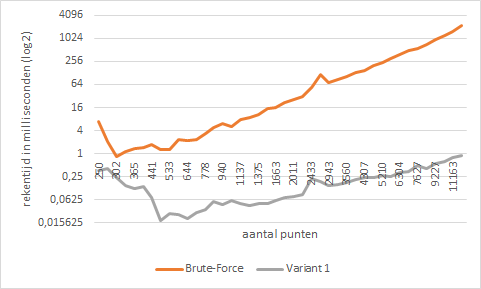
\includegraphics[width=\textwidth]{Simpel-var1-rekentijd.png}
\caption{De plot van de rekentijden tussen het brute-force algoritme en variant 1}
\end{figure}

\begin{figure}
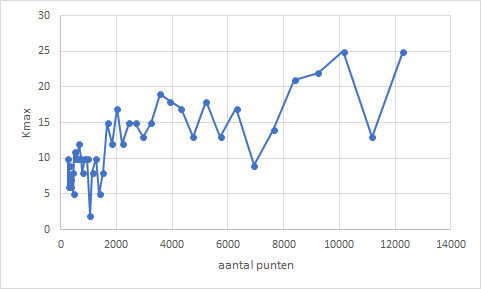
\includegraphics[width=\textwidth]{punten-Kmax.png}
\caption{De plot tussen het aantal punten en Kmax}
\end{figure}

\begin{figure}
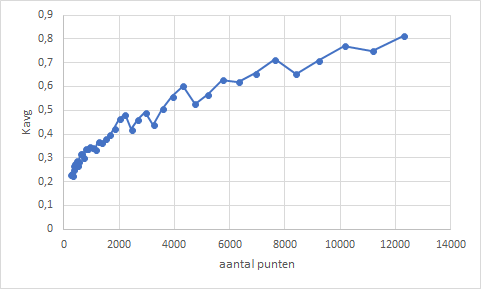
\includegraphics[width=\textwidth]{punten-Kavg}
\caption{De plot tussen het aantal punten en Kavg}
\end{figure}

\begin{figure}
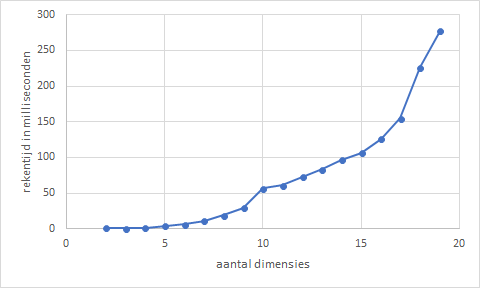
\includegraphics[width=\textwidth]{dim-var1-rekentijd.png}
\caption{De plot tussen het aantal dimensies en de rekentijd van variant 1}
\end{figure}

\begin{figure}
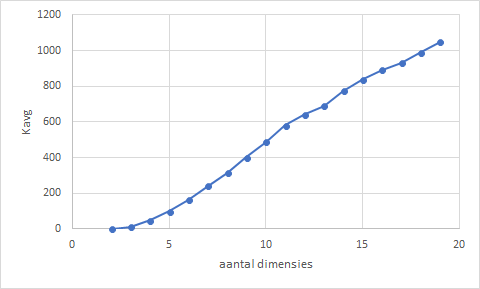
\includegraphics[width=\textwidth]{dim-Kavg.png}
\caption{De plot tussen het aantal dimensies en Kavg}
\end{figure}







\end{document}
